Table~\ref{tab:compare} compares hybrid QAOA with standard methods over all 12 periods. Every stochastic method was run with 20 random seeds per period (240 runs). Methods that work on the QUBO (exhaustive search, SA and QAOA) all evaluate 4096 bitstrings and refine their five lowest-energy candidates in exactly the same way, so they differ only in how they search the binary space. PSO and GA work on the continuous outputs with a similar budget (3030 evaluations).

\begin{table}[H]
\centering
\caption{Comparison with standard algorithms (12 periods; 20 seeds each for stochastic methods). Success: within 0.1\,\% of SLSQP and $|\text{mismatch}| \le 0.01$~MW.}
\label{tab:compare}
\small
\begin{tabular}{llrrrr}
\toprule
Method & Space & Mean gap & Worst gap & Success & Time/period\\
\midrule
SLSQP (reference) & continuous & 0 & 0 & 100\,\% & 1.3 ms\\
$\lambda$-iteration & continuous & 0 & 0 & 100\,\% & 0.5 ms\\
PSO, dep.\ unit \cite{gaing2003} & continuous & 0.0000\,\% & 0.0003\,\% & 100\,\% & 13 ms\\
GA, dep.\ unit & continuous & 0.0000\,\% & 0.0001\,\% & 100\,\% & 80 ms\\
PSO, penalty & continuous & 0.645\,\% & 2.190\,\% & 13.8\,\% & 10 ms\\
GA, penalty & continuous & 0.763\,\% & 3.011\,\% & 7.5\,\% & 81 ms\\
Exhaustive + refine & 12-bit QUBO & 0.007\,\% & 0.040\,\% & 100\,\% & 10 ms\\
SA + refine & 12-bit QUBO & 0.029\,\% & 0.437\,\% & 92.5\,\% & 71 ms\\
\textbf{QAOA + refine} & 12-bit QUBO & \textbf{0.007\,\%} & \textbf{0.040\,\%} & \textbf{100\,\%} & 0.28 s$^\dagger$\\
\bottomrule
\multicolumn{6}{l}{\footnotesize $^\dagger$ Sampling on a laptop simulator, after about 22~s of training per period.}
\end{tabular}
\end{table}

\begin{figure}[H]
\centering
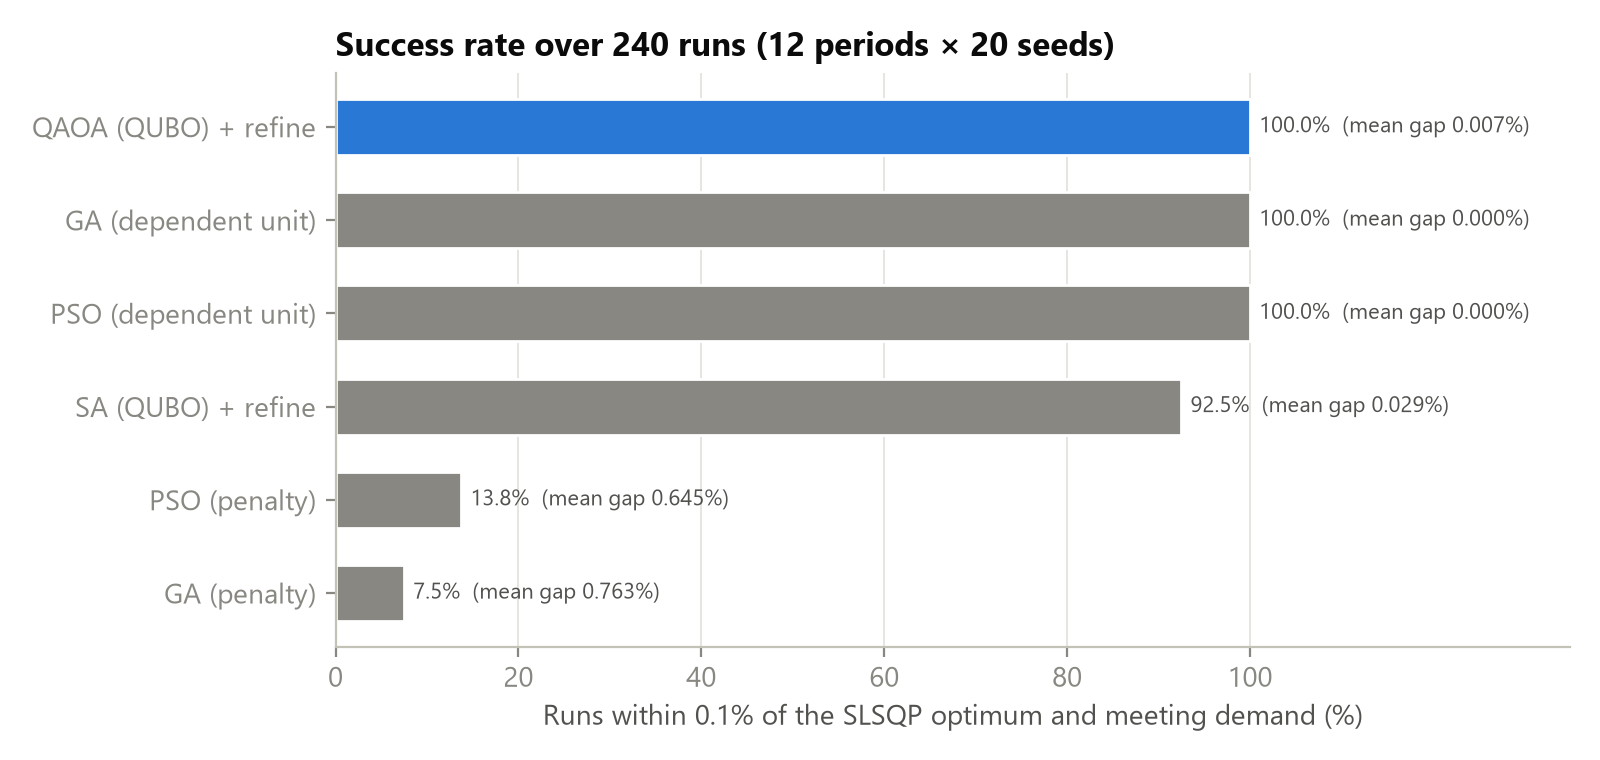
\includegraphics[width=0.9\textwidth]{baselines_success}
\caption{Success rate of the stochastic methods over 240 runs.}
\label{fig:baselines}
\end{figure}

The comparison shows the following.
\begin{itemize}
\item \textbf{Against the same binary problem}, QAOA performed as well as exhaustive search in every one of the 240 runs, with identical costs. Simulated annealing with the same budget and the same refinement succeeded in 92.5\,\% of runs, with a worst gap of 0.44\,\%. On this problem QAOA's sampling was therefore more reliable than SA.
\item \textbf{The 0.007\,\% mean gap of QAOA is a property of the 4-bit grid}, not of QAOA: exhaustive search, which by definition finds the QUBO optimum, gives the same value.
\item \textbf{Continuous heuristics} reach the exact optimum when the balance constraint is handled by the dependent-unit method of Gaing \cite{gaing2003}, because they are not limited to a grid. With a plain penalty they often stop at a nearby but more expensive dispatch (13.8\,\% and 7.5\,\% success). This shows that constraint handling matters as much as the choice of algorithm.
\item \textbf{Speed:} every classical method is faster than simulated QAOA. Simulating a quantum circuit on a classical computer costs time that grows exponentially with the number of qubits, so no runtime advantage can be expected here.
\end{itemize}
